\documentclass[a4paper,11pt]{article}
\usepackage[utf8]{inputenc}
\usepackage[T1]{fontenc}
\usepackage[x11names,table]{xcolor}
\usepackage[french]{babel}
\usepackage{wasysym}
\usepackage{natbib}
% Si l'on veut produire une version PDF avec distiller ou pdflatex:
\usepackage[pageanchor=false,colorlinks,plainpages=false]{hyperref}
\usepackage{url}

\ifx\pdftexversion\undefined
\usepackage[dvips]{graphicx}
\else
\usepackage[pdftex]{graphicx}
\DeclareGraphicsRule{*}{mps}{*}{}
\fi

\graphicspath{{Images/}}

\usepackage{time}
%\usepackage[scaled]{helvet}
%\renewcommand*\familydefault{\sfdefault} %% Only if the base font of the document is to be sans serif

\usepackage{listings}
\usepackage{todonotes}
\usepackage{tikz-er2}
\usepackage{pgf-umlcd}
\usetikzlibrary{decorations.text}
\usetikzlibrary{decorations.markings}
\usetikzlibrary{positioning}
\usetikzlibrary{shadows}
\usetikzlibrary{backgrounds}
\tikzstyle{every entity} = [top color=white, 
                            bottom color=blue!30, 
                            draw=blue!50!black!100, 
                            drop shadow]
\tikzstyle{every weak entity} = [drop shadow={shadow xshift=.7ex, shadow yshift=-.7ex}]
\tikzstyle{every attribute} = [top color=white, 
                               bottom color=yellow!20, 
                               draw=yellow, 
                               node distance=1cm, 
                               drop shadow]
\tikzstyle{every relationship} = [top color=white, 
                                  bottom color=yellow!20,  
                                  draw=yellow, 
                                  drop shadow]
\tikzstyle{every isa} = [draw=blue!50!black!100]

\usepackage[]{subfig}
%\renewcommand{\thesubfigure}{Figure~\thefigure.\arabic{subfigure}}
%\captionsetup[subfigure]{labelformat=simple,labelsep=colon, listofformat=subsimple}
%\captionsetup{lofdepth=2}
%\makeatletter
%\renewcommand{\p@subfigure}{}
%\makeatother

\usepackage{geometry}
\geometry{%
a4paper,
body={160mm,250mm},
left=25mm,top=20mm,
headheight=7mm,headsep=4mm,
marginparsep=3mm,
marginparwidth=27mm}

\usepackage{changepage}
\usepackage{placeins}

\usepackage{rotating}

\newenvironment{agrandirmarges}[2]{%
\begin{list}{}{%
\setlength{\topsep}{0pt}%
\setlength{\listparindent}{\parindent}%
\setlength{\itemindent}{\parindent}%
\setlength{\parsep}{0pt plus 1pt}%
\checkoddpage%
\ifoddpage
\setlength{\leftmargin}{-#1}\setlength{\rightmargin}{-#2}
\else
\setlength{\leftmargin}{-#2}\setlength{\rightmargin}{-#1}
\fi}\item }%
{\end{list}}

\newcounter{compteurQuestion}
\setcounter{compteurQuestion}{0}
\newcommand{\Question}{\paragraph*{Question~\thecompteurQuestion~:}\addtocounter{compteurQuestion}{1}}

\date{}
\begin{document}
\lstset{
         breaklines=true,
         %frame=ltrb,
         framesep=5pt,
         %samepage=true,
         tabsize=4,
         basicstyle=\normalsize,
         frameround=ftft,
         keywordstyle=\ttfamily\color{SeaGreen4},
         identifierstyle=\ttfamily\bfseries\color{RoyalBlue4},
         commentstyle=\color{RoyalBlue3},
         stringstyle=\ttfamily,
         showstringspaces=false
}
\pgfdeclarelayer{background}
\pgfdeclarelayer{foreground}
\pgfsetlayers{background,main,foreground}

\newlength{\niveauZero}
\newlength{\niveauUn}
\newlength{\niveauDeux}
\newlength{\niveauTrois}
\newlength{\niveauQuatre}
\newlength{\niveauCinq}

\newlength{\colonneZero}
\newlength{\colonneUn}
\newlength{\colonneDeux}
\newlength{\colonneTrois}
\newlength{\colonneQuatre}
\newlength{\colonneCinq}


{\centering
    \mbox{
      \makebox[15cm][l]{
      \begin{minipage}{15cm}
        \begin{center}
          {\Huge Introduction à JDBC} \\[1cm]
          {\Large Sébastien \textsc{Nedjar} et Fabien \textsc{Pesci}}
        \end{center}
      \end{minipage}
      }
    }
}\\[0.4cm]
\section{Introduction}
L'objectif de ce document est de vous présenter une méthode d'accès à un \textsc{Sgbd} à travers le langage de  
programmation Java. Pour cela, nous allons dans un premier temps présenter l'API JDBC (Java DataBase  
Connectivity)\footnote{\url{http://download.oracle.com/javase/6/docs/technotes/guides/jdbc/}}. C'est un ensemble de  
classes permettant d'exécuter des ordres \textsc{Sql} de manière générique. En effet, l'API JDBC est construit autour 
de pilotes (Driver) interchangeables. Un pilote est un module logiciel  dédié à une source de données (un 
\textsc{Sgbd-R} dans la plupart des cas). Pour utiliser comme source de  données MySQL au lieu d'Oracle, il suffit de de
 remplacer le pilote Oracle par celui de MySQL.  Ce changement de pilote peut se faire directement par paramétrage sans 
 même avoir besoin changer une seule ligne  de code ni même le recompiler\footnote{Il faut tout de même pondérer ces 
 avantages car dans la pratique il existe  de très nombreuses incompatibilités liées à des implémentations du langage 
 \textsc{SQL} non respectueuses des standards.}.

\section{Mise en place de l'environnement de travail}

L'API JDBC fait partie de Java mais le pilote propre au \textsc{Sgbd-R} Oracle n'y est pas. Avant de pouvoir se connecter 
à la base de données située sur \emph{allegro}, il faudra donc ajouter à votre projet le fichier \emph{jar} contenant le pilote 
adapté. Le prochain paragraphe sera consacré à l'installation de ce fichier à partir de l'IDE Eclipse.

Avant de commencer, récupérez l'un des pilotes dans le repertoire local : \url{/commun/nedjar/ojdbc6.jar} ou 
\url{/commun/nedjar/mysql-connector-java-5.1.23-bin.jar}. 
Placer le fichier dans répertoire \url{~/net-home/tp/tpBDA/}. Puis à partir d'Eclipse, lancez 
l'assistant de création de nouveau projet Java (\texttt{File $\rightarrow$ New $\rightarrow$ Java Project}).
Après avoir rempli les informations de ce premier écran, validez pour passer au suivant (\emph{cf.} Figure~\ref{capture1}).
Dans la nouvelle fenêtre, cliquez sur l'onglet \emph{Libraries} (\emph{cf.} Figure~\ref{capture2})
puis sur le bouton \emph{Add External JARs} (\emph{cf.} Figure~\ref{capture3}), sélectionnez le fichier \texttt{ojdbc14.jar} 
précédemment téléchargé (\emph{cf.} Figure~\ref{capture4}), validez en cliquant sur \emph{Finish}. Une fois ces étapes validées, 
vous avez un projet java capable d'utiliser JDBC pour interagir avec Oracle.
\begin{figure}\centering
  \begin{agrandirmarges}{1cm}{1cm}
    \subfloat[][Premier écran de l'assistant création de nouveau projet Java\label{capture1}]{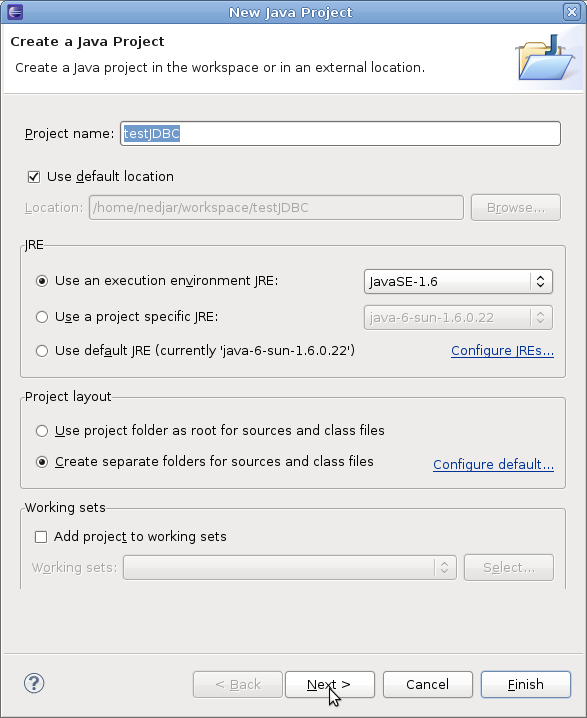
\includegraphics[width=0.48\linewidth]{capture1}}%
    \hfill%
    \subfloat[][Deuxième écran de l'assistant création de nouveau projet Java\label{capture2}]{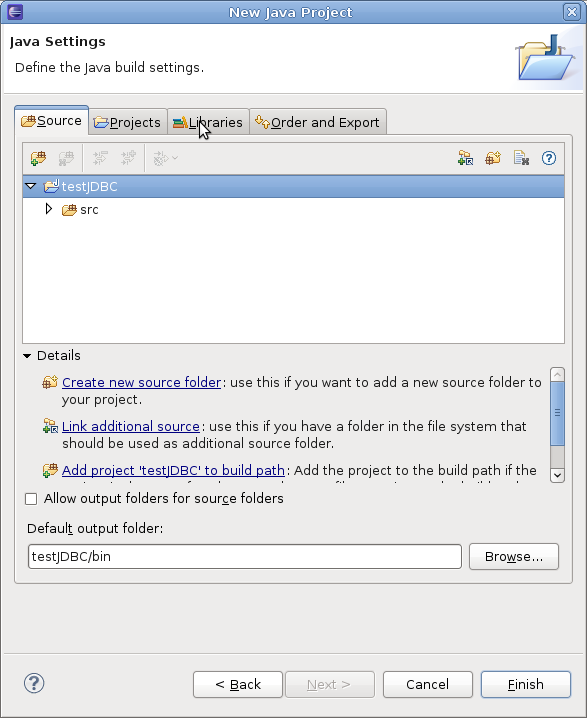
\includegraphics[width=0.48\linewidth]{capture2}}\\

    \subfloat[][Onglet \emph{Libraries} \label{capture3}]{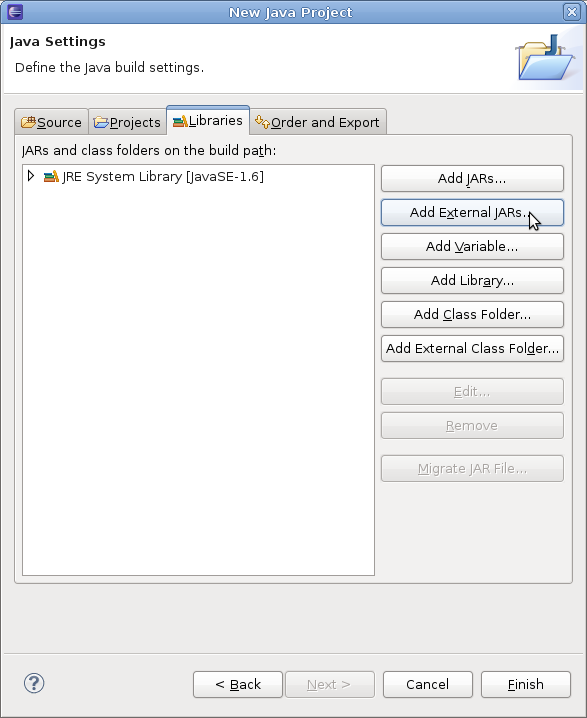
\includegraphics[width=0.48\linewidth]{capture3}}%
    \hfill%
    \subfloat[][Fenêtre de selection du fichier \url{~/net-home/tp/tpBDA/ojdbc6.jar} \label{capture4}]{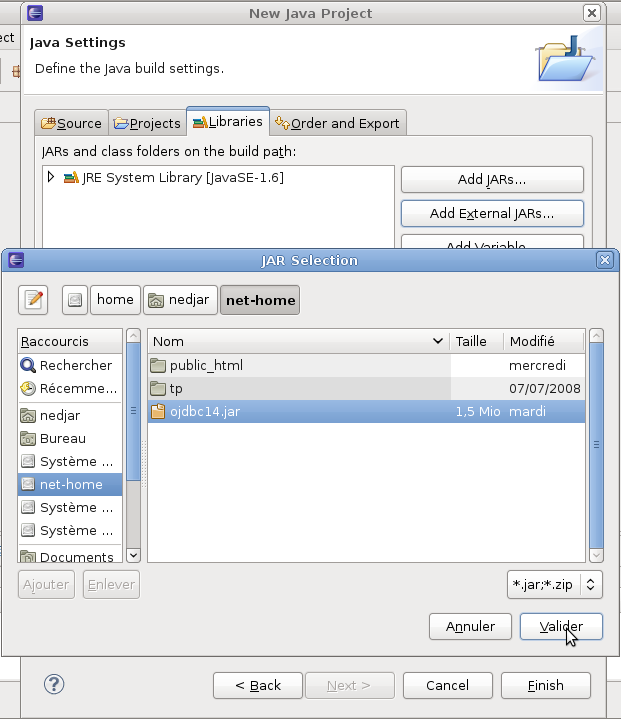
\includegraphics[width=0.48\linewidth]{capture4}}%
    \caption{}
  \end{agrandirmarges}
\end{figure}

\section{Traitement d'un ordre \textsc{Sql} avec JDBC}
L'objectif général de cette partie est de mettre en évidence le schéma de fonctionnement 
classique de l'API Java d'interaction avec les bases de données relationnelles. 
Le principe de fonctionnement de cette API est proche de celle de PHP ou de C\#.
D'une manière générale, pour traiter un ordre \textsc{Sql} avec JDBC, il faudra suivre les 
étapes suivantes :
\begin{enumerate}
  \item Connexion à la base de données.
  \item Création d'une instruction \textsc{Sql}.
  \item Exécution de la requête.
  \item Traitement de l'ensemble des résultats.
  \item Libération des ressources et fermeture de la connexion.
\end{enumerate}
Étant donné que chacune de ses étapes est susceptible de rencontrer des erreurs, il faudra donc rajouter une
étape supplémentaire de gestion des exceptions. 

Pour illustrer ce propos, nous utiliserons la base de données «~Gestion 
Pédagogique\footnote{Script de régénération disponible à l'adresse suivante : 
\url{/commun/nedjar/gestion_peda_oracle.sql} ou \url{/commun/nedjar/gestion_peda_mysql.sql}}~» que vous avez 
utilisée lors de vos TP de \textsc{Pl/Sql} en début d'année. Le modèle conceptuel des 
données est rappelé par la figure~\ref{mcd_gestion_peda}.


\begin{figure}\centering
\begin{tikzpicture}[node distance=1.96cm, every edge/.style={link}]

  \node[entity] (mat) {
    \textbf{Module}
    \nodepart{second}
    \key{Code}\\
    Libellé\\
    H\_Cours\_Prev\\
    H\_Cours\_Rea\\
    H\_TP\_Prev\\
    H\_TP\_Rea\\
    Discipline\\
    Coef\_Test\\
    Coef\_CC\\
  };

  \node[entity] (etud) [below right =of mat ] {
    \textbf{Etudiant}
    \nodepart{second}
    \key{Num\_Et}\\
	  Nom\_Et\\
	  Prénom\_Et\\
	  CP\_Et\\
	  Ville\_Et\\
	  Année\\
	  Groupe\\
  };

  \node[entity] (ens) [above right=of etud ] {
    \textbf{Prof}
    \nodepart{second}
    \key{Num\_Prof}\\
	  Nom\_Prof\\
	  Prénom\_Prof\\
	  Adr\_Prof\\
	  CP\_Prof\\
	  Ville\_Prof\\
  };

  \node[relationship] (notation) [below =of mat] {Notation}
     child {node[attributes] {Moy\_CC\\Moy\_Test}};
  \draw[link] (mat) -- node [pos=0.15, auto] {(0,n)} (notation);
  \draw[link] (etud.145) -- node [pos=0.35, auto, swap] {(0,n)} (notation);

  \node[relationship] (enseigne) [above=of etud] {Enseignement};  
  \draw[link] (mat.315) -- node [pos=0.40, auto] {(0,n)} (enseigne.west);
  \draw[link] (ens.208) -- node [pos=0.40, auto, swap] {(0,n)} (enseigne.east);
  \draw[link] (etud) -- node [pos=0.15, auto, swap] {(0,n)} (enseigne);

  \node[relationship] (mat_spec) [above=1cm of enseigne] {Spécialiste};
  \draw[link] (mat.12) -- node [pos=0.35, auto] {(0,n)} (mat_spec);
  \draw[link] (ens.145) -- node [pos=0.35, auto, swap] {(1,1)} (mat_spec);
  
  \node[relationship] (resp) [above=1cm of mat_spec] {Responsable};
  \draw[link] (mat.56) -- node [pos=0.3, auto] {(1,1)} (resp);
  \draw[link] (ens.north) |- node [pos=0.15, auto, swap] {(0,n)} (resp.east);

  \node[relationship] (mat_pere) [left=1cm of mat] {A pour père};
  \draw[link] (mat.150) -| node [pos=0.1, auto, swap] {(1,1)} (mat_pere.north);
  \draw[link] (mat.210) -| node [pos=0.1, auto] {(0,n)} (mat_pere.south);
  
\end{tikzpicture}
\caption{Modèle conceptuel des données de la base «~Gestion Pédagogique~»\label{mcd_gestion_peda}}
\end{figure}

Le programme Java ci-dessous\footnote{Code source disponible à l'adresse suivante : 
\url{/commun/nedjar/testJDBC.java}} va être utilisé pour illustrer le fonctionnement de chacune 
de ces étapes. L'objectif de ce programme est de récupérer la liste des numéros, noms et prénoms de tous les étudiants 
habitant à Aix-en-Provence pour l'afficher à l'écran. Cet exemple utilise un driver propre à 
Oracle. Il faudrait le remplacer par un autre pour utiliser un \textsc{Sgbd} différent.
\pagebreak
\begin{lstlisting}[language=java]
// Ne pas faire un copier/coller du pdf...

// Importer les classes jdbc
import java.sql.*;

public class testJDBC {
	// Chaine de connexion
	static final String CONNECT_URL = "jdbc:mysql://localhost:3306/maBD";
	static final String LOGIN = "monLogin";
	static final String PASSWORD = "monPaswd";
	// La requete de test
	static final String req = "SELECT NUM_ET, NOM_ET, PRENOM_ET " +
	                          "FROM ETUDIANT " +
	                          "WHERE VILLE_ET = 'AIX-EN-PROVENCE'";                                     
	public static void main(String[] args) throws SQLException {
		// Objet materialisant la connexion a la base de donnees
		Connection conn = null;
		try {
			// Connexion a la base
			System.out.println("Connexion a " + CONNECT_URL );
			conn = DriverManager.getConnection(CONNECT_URL,LOGIN,PASSWORD);
			System.out.println("Connecte\n");
			// Creation d'une instruction SQL
			Statement stmt = conn.createStatement();
			// Execution de la requete
			System.out.println("Execution de la requete : " + req );
			ResultSet rset = stmt.executeQuery(req);
			// Affichage du resultat
			while (rset.next()){	
				System.out.print(rset.getInt("NUM_ET") + " ");
				System.out.print(rset.getString("NOM_ET") + " ");
				System.out.println(rset.getString("PRENOM_ET"));
			}
			// Fermeture de l'instruction (liberation des ressources)
			stmt.close();
			System.out.println("\nOk.\n");
		} catch (SQLException e) {
			e.printStackTrace();// Arggg!!!
			System.out.println(e.getMessage() + "\n");
		} finally {
			if (conn != null) {
				// Deconnexion de la base de donnees
				conn.close();
			}
		}
	}
}
\end{lstlisting}
Les différentes étapes détaillées ci-dessous mentionnent de nombreuses classes contenues dans les paquetages 
\texttt{java.sql.*} et \texttt{javax.sql.*}. Pour connaître les détails sur chacune de ces classes vous êtes 
invités à lire la Javadoc que vous trouverez à l'adresse suivante : \url{http://download.oracle.com/javase/6/docs/api/}.

\subsection{Connexion à la base de données}
La première étape qui permet d'interagir avec une base de données est la connexion. Il faut initialiser 
un objet du type \texttt{Connection} grâce à la méthode \texttt{getConnection()} de la classe \texttt{DriverManager}.

\subsection{Création d'une instruction \textsc{Sql}}
Une fois la connexion établie, il faut créer un objet matérialisant l'ordre \textsc{Sql} à exécuter. Cet objet 
du type \texttt{Statement} est obtenu en appelant la méthode \texttt{createStatement()} de notre connexion.
Il existe trois types d'ordre : 
\begin{enumerate}
	\item Les \texttt{Statement} : Ils permettent d'exécuter n'importe quelle requête sans paramètre. La requête est 
	interprétée par le \textsc{Sgbd} au moment de son exécution. Ce type d'ordre est à utiliser principalement 
	pour les requêtes à usage unique.
	\item Les \texttt{PreparedStatement} : Ils permettent de précompiler un ordre avant son exécution. Ils sont 
	particulièrement importants pour les ordres destinés à être exécutés plusieurs fois comme par exemple les 
	requêtes paramétrées.
	\item Les \texttt{CallableStatement} : Ils sont destinés à l'appel des procédures stockées.
\end{enumerate}

\subsection{Exécution de la requête}
Afin d'exécuter une requête, il suffit de faire appel à l'une des méthodes \texttt{executeXXXX()} de l'objet \texttt{Statement} 
que l'on vient de créer. Dans l'exemple ci-dessus on utilise la méthode \texttt{executeQuery()} en lui passant 
en paramètre une chaîne de caractères (\texttt{string}) contenant la requête (comme \textsc{Execute Imediate} 
de \textsc{Pl/Sql}). Cette méthode retourne un objet du type \texttt{ResultSet} contenant l'ensemble des résultats de la 
requête. Il faut noter que si l'ordre \textsc{Sql} est une mise à jour des données (\textsc{Insert}, 
\textsc{Update}, \textsc{Delete}), il faudra alors l'exécuter avec la méthode \texttt{executeUpdate()} qui 
retourne un entier correspondant au nombre de lignes impactées par la mise à jour.

\subsection{Traitement de l'ensemble des résultats}
La manipulation du résultat d'une requête se fait à travers un objet du type \texttt{ResultSet}.
Le résultat se manipule, comme avec les curseurs de \textsc{Pl/Sql}, ligne après ligne. Ainsi, l'objet 
\texttt{ResultSet} maintient un pointeur vers la ligne courante. La manipulation de ce pointeur se fait avec la 
méthode \texttt{next()} qui permet d'avancer le pointeur sur la ligne suivante. Lors de la création 
du \texttt{ResultSet} ce pointeur est positionné sur une ligne spéciale appelée le \emph{gap}. Cette ligne 
est située une ligne avant la première ligne du résultat. De ce fait, la première ligne n'est pointée  qu'après le 
premier appel à \texttt{next()}. Lorsque le pointeur est positionné après la dernière ligne, \texttt{next()} retourne 
la valeur \texttt{false}. Pour parcourir linéairement l'intégralité d'un \texttt{ResultSet}, on 
utilise donc une boucle \texttt{while} avec \texttt{next()} comme prédicat de continuation. Le corps de 
la boucle est dédié à la manipulation de la ligne (tuple) couramment pointée.

Afin de récupérer les valeurs des attributs du tuple courant, on utilise l'une des différentes 
méthodes \texttt{getXXXX()} (où \texttt{XXXX} désigne le type de l'attribut que l'on 
souhaite récupérer). Par exemple, pour récupérer un entier on utilise \texttt{getInt()} et 
pour récupérer un booléen on utilise \texttt{getBoolean()}. Le paramètre passé à cet accesseur 
permet de choisir l'attribut à récupérer. Il existe deux façons pour désigner un attribut. 
La première (celle de l'exemple) consiste à utiliser une \texttt{string} contenant le nom 
de la colonne souhaitée. La seconde quant à elle, passe en paramètre un entier (\texttt{int}) contenant la position (dans le \textsc{Select}) 
de l'attribut à récupérer. Attention, contrairement à l'habitude en programmation, les attributs 
sont numérotés à partir de 1 (et non de 0). Par exemple, si l'on souhaite récupérer la valeur 
de l'attribut \texttt{NUM\_ET} (le premier dans notre \textsc{Select}), il faudra faire : \texttt{rset.getInt(1)}.

\subsection{Libération des ressources et fermeture de la connexion}
Tant que l'on utilise un \texttt{Statement} ou une \texttt{Connection}, le système nous alloue un certain 
nombre de ressources. Maintenir ces ressources disponibles a un coût non négligeable. Ainsi, comme toujours en 
informatique, pour éviter le gaspillage (et donc un ralentissement inutile) il faut libérer les ressources dès 
qu'elles ne sont plus nécessaires. Pour ce faire, il suffit d'appeler la méthode \texttt{close()} des objets 
\texttt{Statement} et \texttt{Connection}.

\subsection{Gestion des exceptions}
La grande majorité des classes de JDBC sont susceptibles de lever des exceptions lorsqu'elles 
rencontrent des erreurs. C'est pour cela qu'il faut toujours encadrer le code JDBC par un 
bloc \texttt{try/catch}. Les exceptions levées sont toutes des classes filles de \texttt{SQLException}.

\Question Mettre en place un projet TestJDBC pour tester la classe donnée en exemple. 
N'oubliez pas de configurer votre base de données pour qu'elle contienne les données nécéssaires.

\end{document}

